\documentclass[preprint]{aastex}

\usepackage{verbatim}

% A comment block

%\newcommand{\comment}[1]{}

% For color
\newcommand{\mpname}[1]{#1_color.eps}
\newcommand{\clraitoff}{red}
\newcommand{\lumblack}{(black)}
\newcommand{\lumblue}{(blue)}
\newcommand{\lumred}{(red)}
\newcommand{\vdisred}{(red-dashed curve)}
\newcommand{\vdisblue}{(blue-solid curve)}

% For bw
%\newcommand{\mpname}[1]{#1.eps}
%\newcommand{\clraitoff}{}
%\newcommand{\lumblack}{}
%\newcommand{\lumblue}{}
%\newcommand{\lumred}{}
%\newcommand{\vdisred}{(dashed curve)}
%\newcommand{\vdisblue}{(solid curve)}

\newcommand{\umag}{$u$}
\newcommand{\gmag}{$g$}
\newcommand{\rmag}{$r$}
\newcommand{\imag}{$i$}
\newcommand{\zmag}{$z$}
\newcommand{\gmr}{$g-r$}



\newcommand{\gammat}{$\gamma_T$}
\newcommand{\gammacross}{$\gamma_\times$}
\newcommand{\deltasig}{$\Delta \Sigma$}
\newcommand{\deltaplus}{$\Delta \Sigma_+$}
\newcommand{\deltacross}{$\Delta \Sigma_\times$}
\newcommand{\deltarho}{$\Delta \rho$}
\newcommand{\movr}{$M(<r)$}
\newcommand{\sigmacrit}{$\Sigma_{crit}$}

\newcommand{\photoz}{photo-z}
\newcommand{\photozs}{photo-zs}

\newcommand{\tlum}{$L^{tot}$}
\newcommand{\tngal}{$N_{gal}^{tot}$}

\newcommand{\lstarlim}{$0.4 L_*$}
\newcommand{\lvir}{$L_{200}$}
\newcommand{\nvir}{$N_{200}$}
\newcommand{\rvir}{$r_{200}^{gals}$}

\newcommand{\ngal}{$N_{gal}$}
\newcommand{\maxbcg}{maxBCG}
\newcommand{\numNgalBins}{12}
\newcommand{\numLumBins}{16}

\newcommand{\tngalAperture}{2$h^{-1}$ Mpc}

\newcommand{\photo}{\texttt{PHOTO}}
\newcommand{\astrop}{\texttt{ASTRO}}
\newcommand{\mt}{\texttt{MT}}
\newcommand{\spectro}{\texttt{SPECTRO}}
\newcommand{\spectroone}{\texttt{SPECTRO1d}}
\newcommand{\spectrotwo}{\texttt{SPECTRO2d}}
\newcommand{\target}{\texttt{TARGET}}

\newcommand{\lenszmax}{0.3}
\newcommand{\lenszmin}{0.05}

\newcommand{\photoversion}{\texttt{v5\_4}}

%\def\eone{e$_1$}
%\def\etwo{e$_2$}
\newcommand{\etan}{e$_+$}
\newcommand{\erad}{e$_\times$}
\newcommand{\eclass}{\texttt{ECLASS}}
\newcommand{\eclasscut}{-0.06}
\newcommand{\gmrcut}{0.7}

\newcommand{\hrs}{$^{\mathrm h}$}
\newcommand{\minutes}{$^{\mathrm m}$}

\newcommand{\ugriz}{$u, g, r, i, z$}
\newcommand{\polarization}{polarization}

\newcommand{\wgm}{$w_{gm}$}
\newcommand{\wgg}{$w_{gg}^p$}
\newcommand{\wmm}{$w_{mm}$}
\newcommand{\xigg}{$\xi_{gg}$}
\newcommand{\ximm}{$\xi_{mm}$}
\newcommand{\xigm}{$\xi_{gm}$}

\newcommand{\numspec}{127,001}
\newcommand{\numspecvlim}{10,277}
\newcommand{\numrand}{1,270,010}
\newcommand{\numspectot}{278,192}
\newcommand{\numvdis}{49,024}
%\newcommand{\numsource}{10,259,949}
% hirata: 
\newcommand{\nummask}{1,815,043}
\newcommand{\numTenMpc}{132,473}
\newcommand{\numThirtyMpc}{101,221}
\newcommand{\numsource}{27,912,891}

\newcommand{\numpairsTenMpc}{2,670,898,177}
\newcommand{\altnumpairsTenMpc}{2.7 billion}
\newcommand{\numpairsThirtyMpc}{14,818,082,122}
\newcommand{\altnumpairsThirtyMpc}{14.8 billion}



\newcommand{\xirmax}{$\xi_{gm}(R_{max})$}


\newcommand{\modelrmin}{15.0}
\newcommand{\modelrmax}{29.0}
\newcommand{\rmin}{15.0}
\newcommand{\rmax}{21.5}
\newcommand{\pofz}{P$(z$)}
\newcommand{\contam}{unknown}
\newcommand{\nphoto}{unknown}
\newcommand{\ntrain}{unknown}
\newcommand{\matchrad}{2 arcsec}

\def\eps@scaling{1.0}% 

\slugcomment{Last revision \today}
\shortauthors{Sheldon}
\shorttitle{DR8 Photoz Catalog}

\begin{document}

\title{A Photometric Redshift Catalog for SDSS DR8}

\author{
Erin S. Sheldon\altaffilmark{1}
}

\altaffiltext{1}{Brookhaven National Laboratory, Bldg 510, Upton, New York 11973}


\begin{abstract}

We present a catalog of photometric redshifts for galaxies the SDSS DR8 imaging
data.  We use the algorithm presented in \citet{LimaPhotoz08} and
\citet{CunhaPhotoz09} to derive the overall redshift distribution for galaxies
with \rmag$ < $\rmax.  We also use this same method to derive estimated
redshift probability distributions \pofz\ for individual galaxies.  The \pofz\
summed over all galaxies is very similar to that of the overall sample,
suggesting that these individual \pofz\ can be used meaningfully in analyses.
The catalogs are available for download through the SDSS website.  These \pofz\
should be used with care, and we describe their proper use in detail.

\end{abstract}

\section{Method} \label{sec:method}

The algorithm is detailed in \citet{LimaPhotoz08} and \citet{CunhaPhotoz09}.
This method derives weights for a training set of spectroscopically confirmed
galaxies such that the distribution of relevant quantities, such as magnitudes
or colors, matches that of a secondary set of galaxies without known redshifts.
Assuming these quantities correlate with redshift, and are the only relevant
quantities for redshift determination, the resulting weighted redshift
histogram is proportional the redshift probability distribution \pofz\ of the
secondary sample. 


\section{Photometric Data}
Describe DR8.

\section{Photometric Quantities} \label{sec:photo}

In this section we describe the photometric quantities used in creation of the
\photoz\ catalog.  Most of these quantities are measured by the SDSS
photometric pipeline \photo. An early version of the pipeline is described in
\citet{LuptonADASS01}.  Other details can be found in the SDSS Data Release
papers, e.g. \citet{dr4} and at the SDSS website \citep{sdssorg}.  We will give
a few additional details below.

For colors we use the SDSS ``model magnitudes'', which we will refer to as
\modelmag\ \citep{dr7photo}.  Each object is fit to an elliptical exponential
disk, an elliptical \devauc\ profile, and a PSF model determined by
interpolating the PSF to the location of the
object \citep{LuptonADASS01,Sheldon04}.  The exponential and \devauc\ models are
convolved with the local PSF.  For the \modelmag, the best fit model in the
\rmag\ band is then used to extract the flux in the other four bandpasses,
accounting appropriately for the PSF in each band. Thus the effective aperture
is the same for all bands, which is appropriate for extraction of color
information.

We use ``composite model magnitudes'' as an approximate total magnitude for
each object, which we will refer to as \cmodelmag.  For each bandpass
separately, the flux from the best-fitting exponential and \devauc\ models are
combined:
\begin{equation}
\textrm{Flux}_{cmodel} \equiv (1-f_{dev})\times \textrm{Flux}_{exp} + f_{dev} \times \textrm{Flux}_{dev}
\end{equation}
where $f_{dev}$ is the fraction of the total flux estimated to come from a
\devauc\ profile\citep{dr7photo}.  Note the aperture for each band is
different, so these magnitudes are not appropriate for estimating colors.

For quality assurance, we use bits from the \texttt{OBJECT} bitmask output by
\photo.  See \citet{dr7flags} for detailed information about the flags.    We
also use the \texttt{RESOLVE\_STATUS} \citep{dr7resolve} to choose primary
observations.  We will describe how the flags are used in section \S \ref{sec:select}.


\begin{comment}
\begin{itemize}
  \item \texttt{SATUR}  The object contains saturated pixels.
  \item \texttt{BRIGHT} The object is very bright and must be remeasured.
  \item \texttt{DEBLEND\_TOO\_MANY\_PEAKS}
\end{itemize}
\end{comment}
    

\section{Photometric Sample Selection} \label{sec:select}

\subsection{Star Galaxy Separation}

The \photo\ pipeline uses the concentration $c$ to separate stars from
galaxies.  The concentration is the difference between magnitude determined
from the best fitting PSF model \psfmag\ and the best overall fitting model 
\modelmag\ which may or may not be the PSF model.
\begin{equation}
c \equiv \textrm{psfmag} - \textrm{modelmag}
\end{equation}
If the PSF is a good fit to the object, the concentration will be close to
zero, and the object is likely to be a star. The pipeline defines galaxies as
objects with $c > 0.145$ \citep{dr7classify} where $c$ is derived from the
summed fluxes from all bandpasses.  

At our magnitude limit \rmax\ it is estimated that \contam\% of these objects
are actually stars (TODO determine how conservative the algorithm is here?).
Note that for studies where completeness and purity must be known precisely,
\citet{ScrantonMag05} recommend limiting the catalog to \cmodelmag\ less than
21.0 in the \rmag\ band and using more sophisticated star galaxy separation. We
provide a catalog here that should be a superset of objects that can be further
trimmed.

\subsection{Other Cuts}

We remove objects for which the extinction-corrected model flux is not well
determined in at least one of the bands.  The magnitude limits are [21, 22, 22,
20.5, 20.1] for \allmag\ respectively.

In addition to the magnitude limits described above, which only demand a
reasonable detection in at least one band, we additionally demand that we have
detections in both the \rmag\ and \imag\ bands.  Rather than applying a
magnitude cut, we instead use the \texttt{OBJECT} processing flags
\texttt{BINNED}\{1,2,4\}, which indicate the object was detected in the original
image (binned by 1), the 2X2 binned image, or the 4x4 binned image respectively.

We remove all objects that are found to have the following \texttt{OBJECT}
flags set: \texttt{SATUR}, \texttt{BRIGHT}, \texttt{DEBLEND\_TOO\_MANY\_PEAKS},
\texttt{PEAKCENTER}, \texttt{NOTCHECKED}, \texttt{NOPROFILE} as well as objects
that are (\texttt{BLENDED} \&\& \texttt{NODEBLEND}); in other words, detected
to be blended but not successfully deblended into components. 

We only use objects marked as \texttt{SURVEY\_PRIMARY} in their
\texttt{RESOLVE\_STATUS} flags field \citep{dr7resolve}. Different scans on the
sky observe the same objects due to the small overlap regions between adjacent
scans, overlaps at the end of the scan lines where the great circles converge,
and re-observed scan lines.  This results in duplicate observations for many
objects.  These duplicates are ``resolved'' and only a single observation is
kept.

We demand the extinction corrected \citep{Schlegel98} \cmodelmag\ in the \rmag\
band is in the range [\rmin, \rmax].  We also restrict the ordinary \modelmag\
to be within the range [\modelrmin, \modelrmax] in order to ensure reasonable
colors for the galaxies.

We make broad geometrical cuts on the catalog.  We trim the objects to the
\boss\ footprint, shown in figure \ref{fig:footprint}. We also remove any
objects near stars in the tycho2 catalog \citep{tycho2} using a variable radius
that depends on the magnitude of the star:
\begin{equation}
r = (0.0802\times B_T^2 - 1.860\times B_T + 11.625)/60.0
\end{equation}
where $B_T$ is the Tycho magnitude and $r$ is in degrees.  Finally, we remove
all objects from images taken where the \umag\ amplifiers were not working
TODO: ref amplifier.

\begin{figure}[t] \centering
 \centering 
 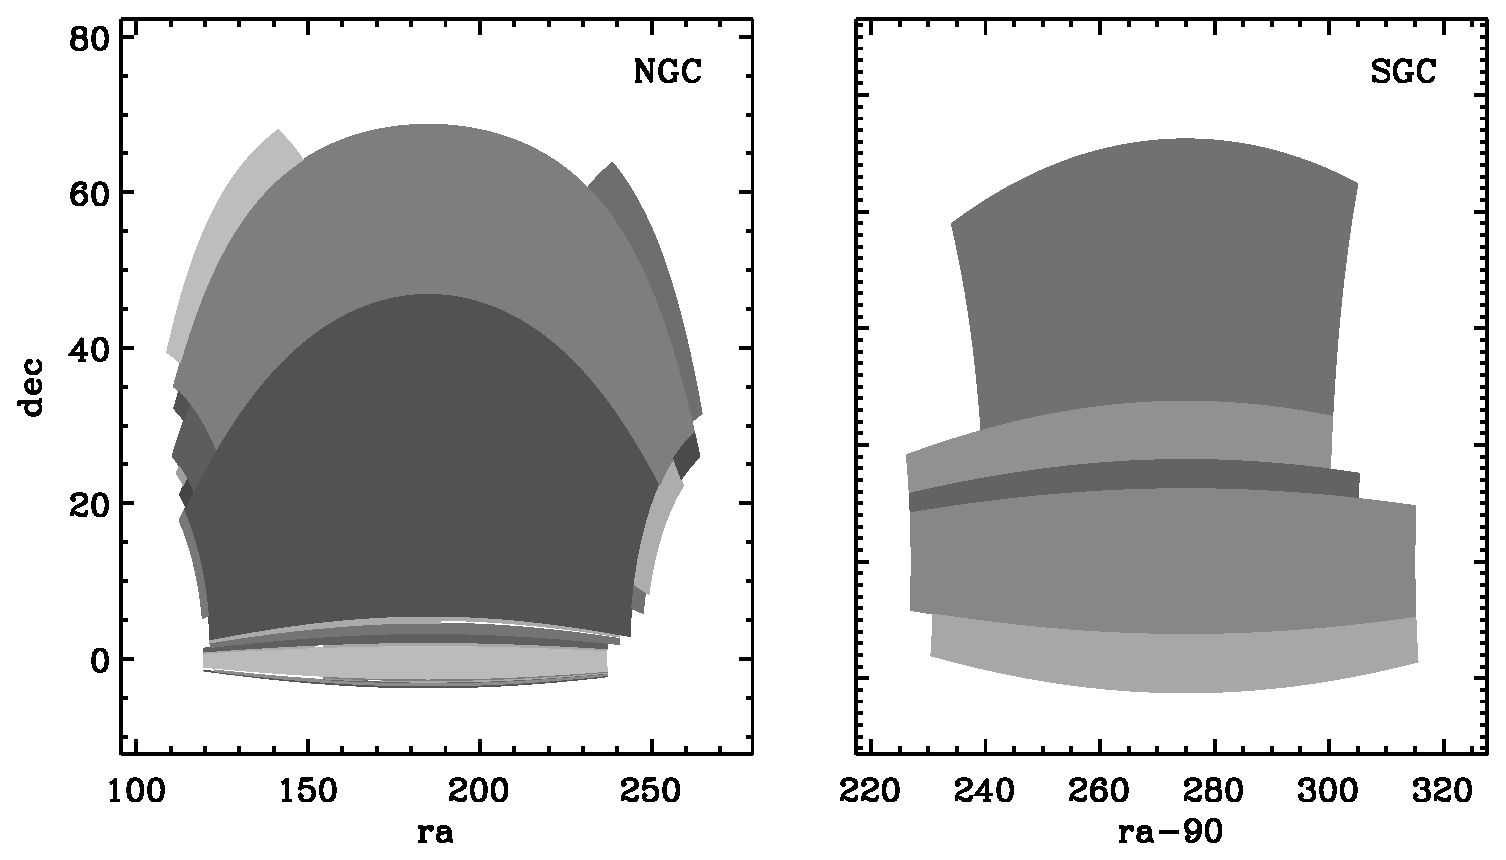
\includegraphics[scale=0.5]{figures/ngc-sgc-poly.eps}
 \caption{BOSS footprint for the north galactic cap on the left
 and the south galactic cap on the right.  The differently shaded
 regions represent contiguous rectangular regions in SDSS survey coordinates.
 Note the plot for the south has been rotated by 90 degrees to avoid
 the split at RA=360.}
 \label{fig:footprint}
\end{figure}

The final photometric catalog contains \nphoto\ objects.  The distribution of
extinction corrected \rmag-band \cmodelmag\ and colors derived from extinction
corrected \modelmag\ are shown in \ref{fig:varhist}.

\section{Training Samples} \label{sec:train}

We use a spectroscopic trining set drawn from a number of sources. These
sources contain mostly galaxies and a small number of stars in order
to help put stellar contaminants from the photometric sample at low
redshift. In the following sections we give short details on each sample
and describe our process for matching to the photometric sample.

\subsection{Samples Used in this Study} \label{sec:train:def}

\begin{itemize} 

    \item 435,897 redshifts from the SDSS spectroscopic sample,
principally from the \texttt{MAIN} and Luminous Red Galaxy \texttt{(LRG)}
samples, with confidence level \texttt{zconf}$ > 0.9$, and r-band
\cmodelmag\ $ <19.5$.


    \item 478 objects from the Canadian Network for Observational
Cosmology (CNOC) Field Galaxy Survey \cite[CNOC2;][]{yee00}\footnote{\tt
http://www.astro.toronto.edu/~cnoc/cnoc2.html} with \texttt{Rval} $>4$
for \texttt{Sc}$=2$ or \texttt{Rval} $> 5$ for \texttt{Sc}$=5$

    \item 184 from the Canada-France Redshift
Survey \cite[CFRS;][]{lilly95}\footnote{\tt
http://www.oamp.fr/people/tresse/cfrs/cfrs.html} with \texttt{Class} $\geq 3$.

    \item 2,199 from the Deep Extragalact Evolutionary Probe 2 survey
\citep[DEEP2;][]{weiner05}\footnote{\tt http://deep.berkeley.edu/DR3}
with \texttt{zqual} $\geq 3$

    \item 234 from the Team Keck Redshift Survey \cite[TKRS;][]{wirth04}\footnote{\tt http://tkserver.keck.hawaii.edu/tksurvey/}.

    \item 8,660 LRGs from the 2dF-SDSS LRG and QSO Survey \cite[2SLAQ;][]{cannon06}\footnote{\tt http://www.2slaq.info/} with \texttt{qop} $\geq$ 3.

    \item  2,252 from zCOSMOS redshift survey \cite{lilly07}, with  \texttt{cc=3.4 || 3.5 || 4.4.  || 4.5 || 9.5}
    
    \item 1,771 from the VIMOS VLT-Deep survey \cite[VVDS;][]{garilli08}\footnote{\tt http://www.oamp.fr/virmos/vvds.htm} with \texttt{zqual} $\geq 3$.

\end{itemize}


\subsection{Matching to SDSS Imaging Data} \label{sec:train:match}

We match by position the training sets listed in \S \ref{sec:train:def} to the
photometric catalog described in \S \ref{sec:select}.  We choose the closest
match within \matchrad.  By performing this match we place the training set
galaxies on the same photometric system as the photometric set.  We also
guarantee that the matches are drawn from the same magnitude range, and
have the same quality cuts applied, as the photometric set.

As noted in \S \ref{sec:train:def}, the training sets contain some stars.
There are also some stars in the photometric set, since the star galaxy
separation is not perfect.  Thus, through this matching between photometric set
and training set it should be possible to place some fraction of the stars in
the photometric set at redshift zero; or at least some part of their derived
\pofz.

\section{Results}

We use the algorithm described in \S \ref{sec:method} to derive weights for
each training set galaxy.  We then use these weights to calculate a weighted
redshift histogram which, under our assumptions, should be proportional to that
of the training set.  We also derive individual redshift probability
distributions \pofz\ for each photometric galaxy.

The \rmag-band \cmodelmag\ and colors based on \modelmag\ for the photometric
and training sets are shown in figure \ref{fig:varhist}.  Also shown are the
derived weights for the training set and the resulting weighted histograms.
The weighted training set distributions should be approximately proportional to
the photometric set distributions in order to derive good redshift
distributions.  There are deviations at \gmr\ $\sim 1.5$ and \rmi\ $\sim 0.6$,
but otherwise the distributions are quite close. TODO Include sub-plots of
the residuals?  Statistical analysis?

\begin{figure}[t] \centering
    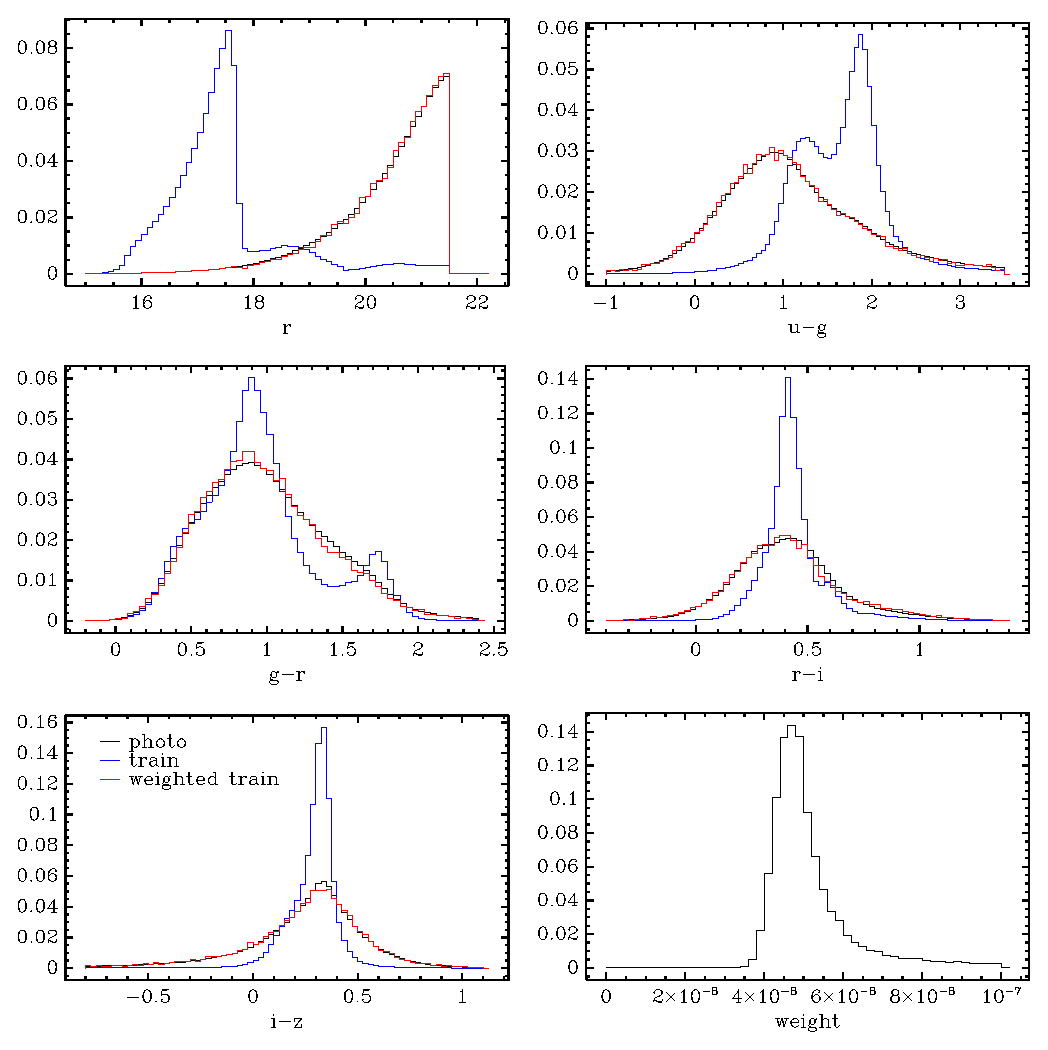
\includegraphics{figures/zweight-09-varhist.eps}

    \caption{Distributions of photometric quantities for the photometric sample
    and training sample.  The upper left panel shows the extinction-corrected
    \rmag-band \cmodelmag.  Note both samples are cut at \rmag$ < $\rmax.  
    Also shown is the weighted histogram for the training sample where
    the weights are derived to produced distributions approximately 
    proportional to the photometric sample.
    The following four panels show extinction corrected colors based on
    \modelmag.  The bottom right panel shows the distribution of the
    derived weights for the training sample.}
    \label{fig:varhist}

    \vspace{2em}
\end{figure}

Figure \ref{fig:pofz} shows the recovered redshift distribution for the entire
\rmag\ $<$ \rmax\ sample.  Also shown is the redshift distribution of the
original training set.  These distributions are in qualitative agreement with
those shown in \citet{CunhaPhotoz09}, although that sample had a fainter \rmag\
limit at 22.0.  Note the sub-plot showing the region near $z=0$.  As expected
there is some fraction of the overall distribution near z=0.  The fraction of
at $z < 0.002$ is about 0.4\%.  It is not known exactly how many stars are in
the photometric sample, but this is probably a lower limit on the stellar
contamination (TODO beef this up).

Also shown in \ref{fig:pofz} is the summed \pofz\ derived for individual
galaxies.  The summed \pofz\ is quite close to that derived for the overall
sample.  This is suggestive that these individual \pofz\ can be used
meaningfully on their own.  TODO: look at the expectation value of the redshift
as a function of true redshift for training set objects?

\begin{figure}[t] \centering
    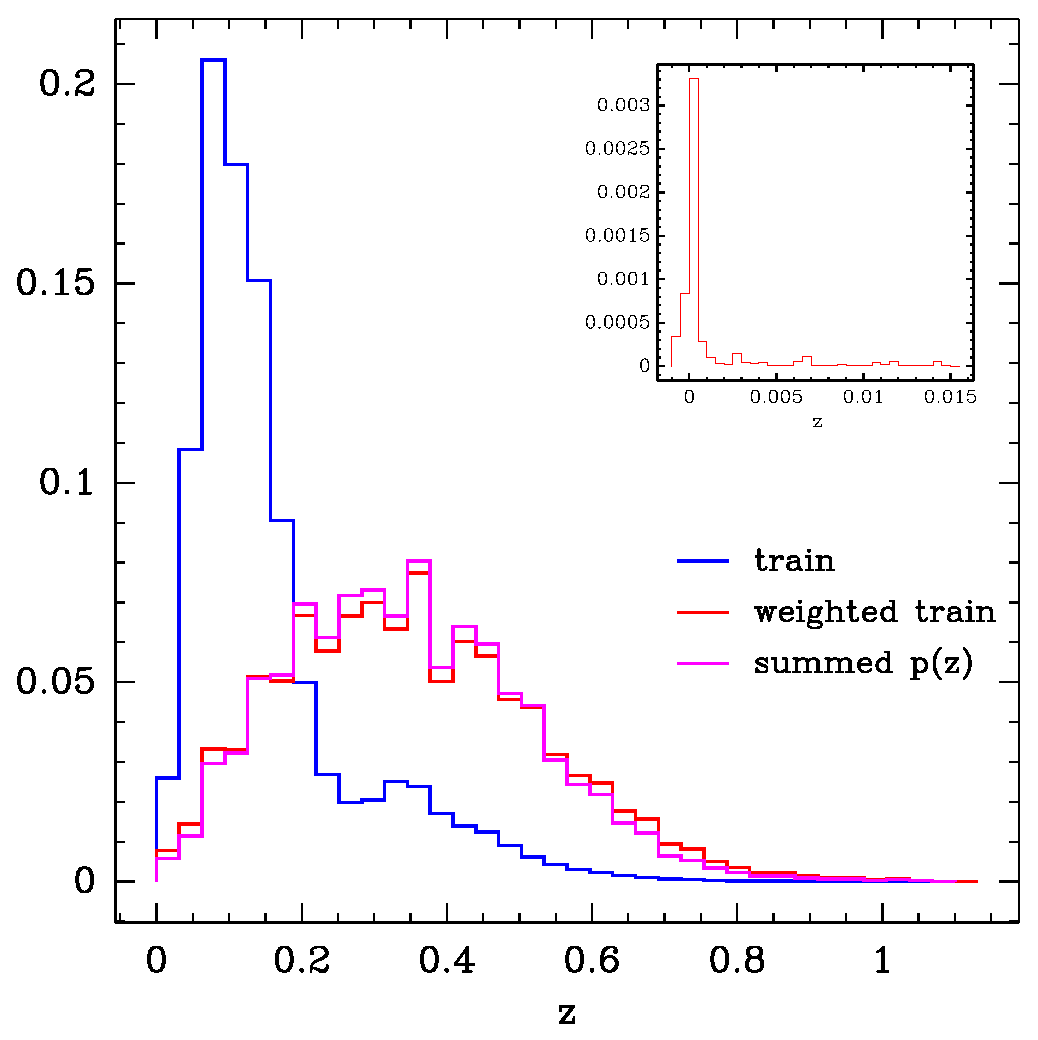
\includegraphics[scale=0.9]{figures/zweight-09-zhist-withorig-withsum-11.eps}

    \caption{Reconstructed redshift distribution for SDSS galaxies with \rmag\
    $ < $ \rmax.  The overall reconstructed distribution, shown in red, is
    derived by creating a weighted histogram of the training set redshifts as
    described in the text.  Also shown in magenta is the sum of all \pofz\
    derived for individual galaxies.  The unweighted training set redshift
    distribution is shown in blue.  The excess at $z \sim 0$ is due to stars in
    training set having signifcant weight; more detail at low redshift is shown
    in the inset.  This excess is at least partly due to the presence of real
    stars in our photometric sample resulting from imperfect star-galaxy
    separation.  The fraction of the distribution at $z < 0.002$ is 0.4\%,
    which is probably a lower bound on the stellar contamination.
    \label{fig:pofz}}

    \vspace{2em}
\end{figure}


\bibliographystyle{apj}
% Bib database
\bibliography{apj-jour,astroref}



\end{document}

